\chapter{Statistical Thoery}
In this chapter we will see some examples of mathematics.

Change title To

Measures, bounds and Hilbert spaces. 

\lipsum[1]

\section{Bounds}

\subsection{Hoeffding}

\subsection{Sanov}

\section{Regression}

\subsection{thoery}

\section{K-means}


\section{Probability metrics}

\subsection{Introduction}

Suppose that we are given samples from two unkown distributions $P$ and $Q$, an 
important question is ask is: do $P$ and $Q$?

We will next see two 


\subsection{f-divergence}

Generalisation of the usual divergence, exploit jensen.

Talk about f-divergence, and give proof that D(p, q) >=0 and eq iff p == q

Talk about IPM vs $f-$divergence. 

To test whether two random variables are independent $X, Y$

talk about L1 being f-divergence


\subsection{Integral Probability Metric}

Observe that if two random variables $X$, $Y$ share the same distribution, then 

$$
\E(g(X)) = \E(g(Y))
$$

for any continuous and bounded function $g : \R \rightarrow \R$. 
It turns out that the reciprocal statement holds.

This motivates the following 

$$
D_\mathcal{H} (P, Q) = 
\sup _{g \in \mathcal{H}} \mid \mathop{\E}_{X \sim P} g(X) - \mathop{\E}_{Y \sim Q} g(Y) \mid
$$

where $\mathcal{F}$ is a class of real-valued bounded measurable functions.

See for example \cite{sriperumbudur2009integral} for a detailed analaysis

This defines a rich class of distance measures known as 
integral probability metrics (IPMs) (see \cite{muller1997integral}). Depending
on how we choose $\mathcal{F}$ we end up with different popular distance measures, such as
the Wasserstein distance or Total variation distance to name a few. 

Note that the variational nature of the measure makes it a hard optimisation problem to tackle.
If we could somehow decompose $g$ linearly into simple components (think Fourier transforms), 
then we could use the linearity of expectation to simplify the problem: this is exactly what
the following restriction achieves.

Consider $\mathcal{F}=\left\{f:\|f\|_{\mathcal{H}} \leq 1\right\}$, this is known
as the maximum mean discrepancy (MMD). Where $\mathcal{H}$, is a reproducing kernel Hilbert space 
(RHKS) with $k$ as its reproducing kernel. 

First note that if $\phi$ is the associated feature map to the kernel $k$ from the associated 
RKHS $\mathcal{H}$ then we have $g(x) = \inp*{g}{\phi(x)} $.

We can thus do the following simplification by linearity of expectation

$$
    \mathop{\E}_{X \sim P} g(X) = 
     \inp*{g}{ \mathop{\E}_{X \sim P} \phi(X)} = \inp*{g}{\mu_P}
$$

Where we have defined\footnote{Note that this is well defined so long as $\phi$ is is continuous and bounded;
one can also show that this object is continuous (See \cite{Peters2008diploma}). Note that 
 $\mu_P \in \mathcal{H}$.}

$$
\mu_P = \mathop{\E}_{X \sim P} \phi(X)
$$

With this simplification and Cauchy Schwartz we have the following chain of equalities

\begin{align*} 
    \text{MMD}_\mathcal{F} (P, Q) 
    &= 
    \sup _{g \in \mathcal{F}} \mid \mathop{\E}_{X \sim P} g(X) - \mathop{\E}_{Y \sim Q} g(Y) \mid \\
    &= 
    \sup _{g \in \mathcal{F}} \mid \inp*{g}{\mu_P - \mu_Q} \mid \\
    &=
    \norm{\mu_P - \mu_Q}_\mathcal{H}
\end{align*}

We can therefore see the MMD as the feature mean difference of the distributions.

We can further simplify the MMD

\begin{align*}
    \text{MMD}_\mathcal{F}^2 (P, Q)
    &=
    \norm{\mathop{\E}_{X \sim P} \phi(X)  - \mathop{\E}_{Y \sim Q} \phi(Y) }_\mathcal{H}^2 \\
    &= \mathop{\E}_{X \sim P} \mathop{\E}_{X^\prime \sim P} \inp*{\phi(X)}{\phi(X^\prime)} - 
    2 \mathop{\E}_{X \sim P} \mathop{\E}_{Y \sim Q} \inp*{\phi(X)}{\phi(Y)} +
    \mathop{\E}_{Y \sim Q} \mathop{\E}_{Y^\prime \sim Q} \inp*{\phi(Y)}{\phi(Y^\prime)} \\
    &= \mathop{\E}_{X \sim P} \mathop{\E}_{X^\prime \sim P} k \left( X, X^\prime \right) - 
    2 \mathop{\E}_{X \sim P} \mathop{\E}_{Y \sim Q} k \left( X, Y \right) +
    \mathop{\E}_{Y \sim Q} \mathop{\E}_{Y^\prime \sim Q} k \left( Y, Y^\prime \right)
\end{align*}

which we can straightforwardly estimate with samples; all the we require is to specify a kernel:
so how do we choose a kernel?

We need to ensure that $\text{MMD}P, Q) = 0$ iff $P = Q$, in other words, $\mu_P$ needs to be injective
as a function of $P$. There are 

We note that HSIC is to MMD, what the Mutual Information is to the Kullback–Leibler divergence.

Benefits -> no bins! 

but this is a lie! HSIC needs to choose a kernel, and the hyperparameters...  

In their study (\cite{sriperumbudur2009integral}) -- it is shown that IPM is much
simpler than estimating f-divergences, and that the estimators
are strongly consistent while exhibiting good rates of conver-
gence. IPMs also account for the properties of
the underlying space M through the Kernel in case of MMD. This is especially
useful when considering disjoint supports between P and Q


% Our study shows that estimating IPMs (especially the
% Wasserstein distance, Dudley metric and MMD) is much
% simpler than estimating φ-divergences, and that the estimators
% are strongly consistent while exhibiting good rates of conver-
% gence. In addition, IPMs also account for the properties of
% the underlying space M (the metric property is determined by
% ρ in the case of Wasserstein and Dudley metrics, while the
% similarity property is determined by the kernel k [37] in the
% case of MMD) while computing the distance between P and
% provide a nice interpretation for IPMs by showing they naturally appear in binary classification. Many previous works [6], [33], [38], [39] relate φ-divergences (between P and Q) to binary classification (where P and Q are the class conditional distributions) as the negative of the optimal risk associated with a loss function (see [40, Section 1.3] for a detailed list of references). In Section IV, we present a series of results that relate IPMs to binary classification. First, in Section IV-A, we provide a result (similar to that for φ-divergences), which shows γF (P, Q) is the negative of the optimal risk associated with a binary classifier that separates the class conditional distributions, P and Q, where the classification rule is restricted to F. Therefore, the Dudley metric, Wasserstein distance, total variation distance and MMD can be understood as the negative of the optimal risk associated with a classifier for which the classification rule is restricted to {f : ∥f∥BL ≤ 1}, {f : ∥f∥L ≤ 1}, {f : ∥f∥∞ ≤ 1} and {f : ∥f∥H ≤ 1} respectively. Next, in Sections IV-B and IV-C, we present a second result that relates the empirical estimators studied in Section III to the binary classification setting, by relating the empirical estimators of the Wasserstein distance and Dudley metric to the margins of the Lipschitz [41] and bounded Lipschitz classifiers, respectively; and MMD to the Parzen window classifier [37], [42] (see kernel classification rule [43, Chapter 10]). The significance of this result is that the smoothness of the classifier is inversely related to the empirical estimate of the IPM between class conditionals P and Q. Although this is intuitively clear, our result provides a theoretical justification.
% Before proceeding with our main presentation, we introduce the notation we will use throughout the paper. Certain proofs and supplementary results are presented in a collection of appendices, and referenced as needed.
% C. Notation
% For a􏰖measurable function f and a signed measure P,
% Pf := f dP denotes the expectation of f under P. 􏰦A􏰧
% represents the indicator function for set A. Given an i.i.d.
% sample X1,...,Xn drawn from P, Pn := 1 n δXi repre- n i=1
% 􏰕
% 3
%  sents the empirical distribution, where δx represents the Dirac measure at x. We use Pnf to represent the empirical expec-
% tation 1 n f(Xi). We define: Lip(M,ρ) := {f : M → n i=1
% 􏰕
%  Q, which is not the case with φ-divergences

%  Advantage, disjoint support 

\section{Reproducing Kernel Hilbert Space}

We will begin by defining the kernel,

\begin{definition}
    Let $\mathcal{X}$ be a non-empty set. A function 
    $k: \mathcal{X} \times \mathcal{X} \rightarrow \R$ is a kernel if 
    \begin{enumerate}
        \item $k$ is symmetric: $k(x, y) = k(y, x)$.
        \item $k$ is positive semi-definite, i.e. $\forall x_1, ..., x_n \in \mathcal{X}$,
        the "Gram Matrix" $K$, defined by $K_{ij} = k(x_i, x_j)$ is positive semi-definite
        \footnote{A matrix $M \in \R^{n\times x}$ is positive semi-definite if $\forall a \in \R^n$
        , $a^\intercal Ma \geq 0$}.
    \end{enumerate}
\end{definition}

It is easy construct new kernels since they are preserved under addition, multiplication and other operations. 
(See for example...)

One example of a kernel -- and one of the most popular ones -- is the Gaussian Kernel defined on $\R^d$:

$$
    k(x, y) = \exp (-\gamma^{-2}\norm{x - y}^2)
$$

Let $\mathcal{X}$ be an arbitrary set and $\mathcal{H}$ a Hilbert space of real valued functions
on $\mathcal{X}$. As per general convention, addition and multiplication are define pointwise:

\begin{equation}
    \begin{array}{lll}
    (\lambda \cdot f)(x) & :=\lambda \cdot f(x) & \forall \lambda \in \R, \forall f \in \mathcal{H} \text { and } \forall x \in \mathcal{X} \\
    (f+g)(x) & :=f(x)+g(x) & \forall f \in \mathcal{H}, \forall g \in \mathcal{H} \text { and } \forall x \in \mathcal{X}
    \end{array}
\end{equation}

% One powerful fact about Hilbert spaces is that every Hilbert space admits an orthonormal basis, 
% and each vectorin the Hilbert space can be expanded as a series in terms of this orthonormal basis.

% For instance L2 blah blah

% $f \in L^1$ then we can decompose $f$ as follows:

% $$
%     f(x) = \int_{-\infty}^{\infty} \hat{f}(\omega) e^{2 \pi i x \omega} d \omega
%     = \inp*{\hat{f}}{\phi(x)}
% $$

We will now take a look at Hilbert spaces whose structure is highly linked with a kernel.

\begin{definition}
    Let $\mathcal{H}$ be a Hilbert space of functions $f: \mathcal{X} \rightarrow \R$. 
    $\mathcal{H}$ is called a Reproducing Kernel Hilbert Space (RKHS) if there is a kernel k such that

    \begin{enumerate}
        \item $ k(x, .) \in \mathcal{H} \quad \forall x \in \mathcal{X}$
        \item $ \inp*{f}{k(x, .)} = f(x) \quad \forall f \in \mathcal{H}$
    \end{enumerate}

\end{definition}

Given the kernel $k$ it is convinient to define the feature map $\phi: \mathcal{X} \rightarrow \mathcal{H}$ as:

$$
    \phi(x) = k(x, .)
$$

The power of this setup -- which is known as the kernel trick -- is that inner product between
features (which can live in very large spaces) are simple function evaluation; 
indeed by letting $f(x) = k(x, x\prime)$ we get

$$
    \inp*{k(x^\prime, .)}{k(x, .)} = k(x, x^\prime)
$$

Observe that both conditions imply that $k$ spans $\mathcal{H}$, i.e.

\begin{equation}
    \mathcal{H}=\overline{\operatorname{span}\{k(\cdot, x): x \in \mathcal{X}\}}
\end{equation}

Indeed is is possible to go the other way around\footnote{See the excellent lecture notes on 
RKHS \cite{BartlettNotes} for more details.} and first define the following vector space

\begin{equation}
    \operatorname{span}(\{\phi(x): x \in \mathcal{X}\})=\left\{f(\cdot)=
    \sum_{i=1}^{n} \alpha_{i} k\left(\cdot, x_{i}\right): n \in \N, x_{i} 
    \in \mathcal{X}, \alpha_{i} \in \R\right\}
\end{equation}

It is possible to equip it with an inner product and to show that it is complete in order to create
a Hilbert Space (at which point we will have created a RKHS).

We will now show case a brief example to illustrate the power of the RHKS. Suppose that we have 
some data say $\{ x_i, y_i\}_{i \in [n]}$; we belive for example $y$ to be a smooth function of $x$.

We can estimate $f$ as follows

\begin{equation}
    f^{*}=\arg \min _{f \in \mathcal{H}}\left(
        \sum_{i=1}^{n} 
        \left(y_{i} - \inp*{f}{\phi\left(x_{i}\right)}_{\mathcal{H}} \right)^{2}
        + \Omega \norm{f}_{\mathcal{H}}^{2}\right)
\end{equation}

An amazing result is that an optimisation of the above form will always admit a representation of the
form -- assuming $\Omega$ is increasing?:

\[
    f^{*} = \sum_{i=1}^{n} \alpha_{i} \phi\left(x_{i}\right)
\]
where $\alpha_{i} \in \mathbb{R}$ for all $1 \leq i \leq n$

This is known as the Representer Theorem. If we wish to approximate a prediction for some $x$,
we can do so as follows:


$$
    f^{*}(x) = \inp*{f^{*}}{\phi\left(x\right)} = 
    \sum_{i=1}^{n} \alpha_{i} \inp*{\phi\left(x_i\right)}{\phi\left(x\right)} =
    \sum_{i=1}^{n} \alpha_{i} k\left(x_i, x\right)
$$

It is precisely because the solution is of this form, that we may exploit the kernel trick. We can
also quickly see what the role of the kernel is. If for example, we $k$ is the Gaussian Kernel, then
the solution will be a linear combination of scaled gaussians centered at the data points
\footnote{In fact this will always be the case when we can write $k\left(x_i, x\right) = k\left(x_i - x\right)$}. 

As a final remark we will explain the role of the penalty $\Omega \norm{f}_{\mathcal{H}}^{2}$; from 
the ML world, we now that this kind of term is known as regularisation and is supposed to help the model 
choose a "simpler" model. This is exactly what is happening, as this term will penalise non-smooth functions.

This can be seen by using Mercer's Theorem -- a Generalisation of the spectral theorem for positive-semidefinite
matrices\footnote{Recall that our Kernel $k$ is a generalisation of a positive-semidefinite Matrix}.

\begin{theorem}[Mercer's] 

Suppose $k$ is a continuous positive semi-definite kernel on a compact set $\mathcal{X}$, then if
, $\forall f \in L_{2}(\mathcal{X})$

\[
\int_{\mathcal{X}} k(u, v) f(u) f(v) d u d v \geq 0
\]

then $k$ has the following decomposition

\begin{equation}
    k(u, v)=\sum_{i=1}^{\infty} \lambda_{i} \psi_{i}(u) \psi_{i}(v)
\end{equation}

Where $\{\psi_i\}$ forms an orthonormal basis of $L_2(\mathcal{X})$, 
such that the corresponding sequence of eigenvalues $\{\lambda_i\}$ are non-negative.

Where the convergence is absolute and uniform, that is,
\[
\lim _{n \rightarrow \infty} \sup _{u, v}\left|k(u, v)-\sum_{i=1}^{n} \lambda_{i} \psi_{i}(u) \psi_{i}(v)\right|=0
\]
    
\end{theorem}

We can now use this decomposition of the Kernel to get further insight, using Mercer's theorem we can 
thus write -- assuming the conditions are met:

$$
    k \left(x, x^{\prime}\right)=\sum_{i=1}^{\infty} 
    \underbrace{\left[\sqrt{\lambda_{i}} \psi_{i}(x)\right]}_{\phi_{i}(x)} 
    \underbrace{\left[\sqrt{\lambda_{i}} \psi_{i}\left(x^{\prime}\right)\right]}_{\phi_{i}\left(x^{\prime}\right)}
$$

We can thus rewrite the solution as follows

$$
    f^{*}(x) = \sum_{i=1}^{n} \alpha_{i} k\left(x_i, x\right) = 
    \sum_{i=1}^{\infty} \phi_i\left(x\right) 
    \sum_{j=1}^{n} \alpha_{j}  \phi_i\left(x_j\right) = 
    \sum_{i=1}^{\infty} \sqrt{\lambda_{i}} \psi_{i}(x) f^{*}_i 
$$

Note that due to the $\Omega \norm{f}_{\mathcal{H}}^{2}$ penalty, $f^{*}_i$ must decay for higher values of $i$. Note that
for example in the Fourier Transform\footnote{Heloo}, in the basis $\{\psi_i\}$, higher values if $i$ correspond to higher 
frequency functions; similarly, for the Gaussian Kernel, higher indicies basis functions correspond to 
higher frequecies. Thus, a higher $\Omega$ will force a faster decay on $f_i$ and thus result in smoother functions
-- in principle, less overfitting. 

\begin{figure}[H]
    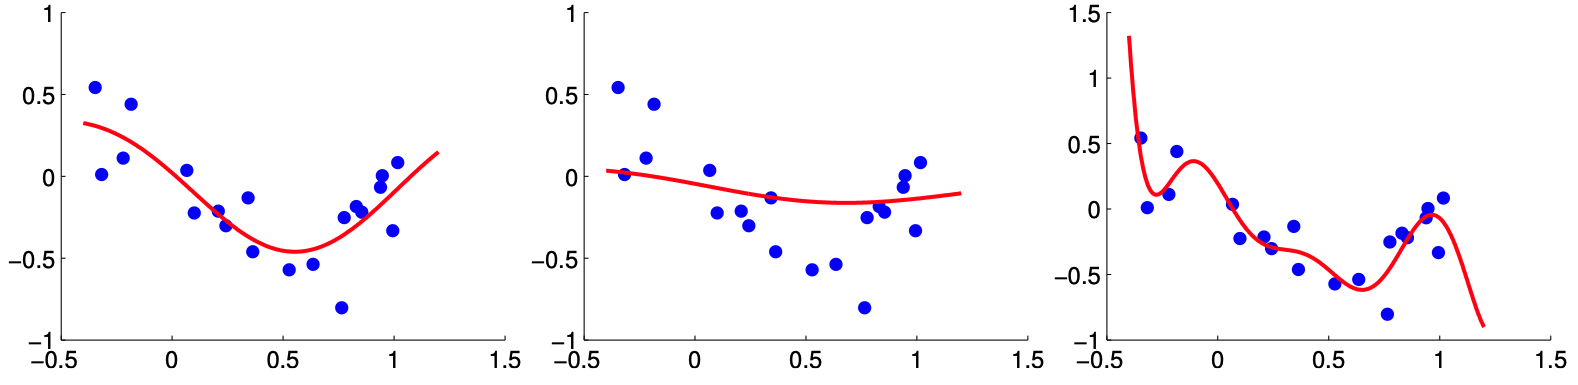
\includegraphics[width=1\textwidth]{kernel_smoothness.jpg}
    \caption{Small RKHS norm results in smooth functions. 
    From left to right $\Omega = .1$, $\Omega = 10$, $\gamma = 1\mathrm{e}{-7}$, 
    we fix the Gaussian kernel with $\gamma = 0.6$}
    \label{fig:kernel_smoothness} 
\end{figure}

% \begin{figure}[tb] 
%     \centering 
%     \includegraphics[width=0.5\columnwidth]{galleria_stampe} 
%     \caption[A floating figure]{A floating figure (the lithograph \emph{Galleria di stampe}, of M.~Escher, got from \url{http://www.mcescher.com/}).}
    
% \end{figure}


